\documentclass{article}
\usepackage{graphicx} % Required for inserting images
\usepackage[utf8]{inputenc}
\usepackage[russian]{babel}
\usepackage{amssymb}
\usepackage{graphicx}
\usepackage{amsmath}
\usepackage[inkscapelatex=false]{svg}
\usepackage{geometry}
\newcommand{\RE}{\mathrm{Re}}
\newcommand{\IM}{\mathrm{Im}}
\usepackage{fancyhdr}
\usepackage{svg}


\geometry{verbose,a4paper,tmargin=2cm,bmargin=2cm,lmargin=2.5cm,rmargin=1.5cm}
\graphicspath{ {./images/} }


\title{Иерархия Кадомцева-Петвиашвили и проблема Шоттки}
\date{}

\fancypagestyle{firstestfirst}{%
  \fancyhf{}%
  \fancyhead[C]{Независимый Московский Университет \\ Математический колледж}
  \fancyfoot[C]{Переведено в формат \LaTeX \ Ваней Фадеевым \\ Высшая школа современной математики (ВШМ) МФТИ, 2026 }
  \renewcommand{\headrulewidth}{0.4pt}
  \renewcommand{\footrulewidth}{0.4pt}
}

\author{Е. Е. Демидов}



\def\svgwidth{0.55\textwidth} 












\begin{document}


\maketitle
\thispagestyle{firstestfirst}

\begin{center}
\textit{Специальный курс}
\end{center}


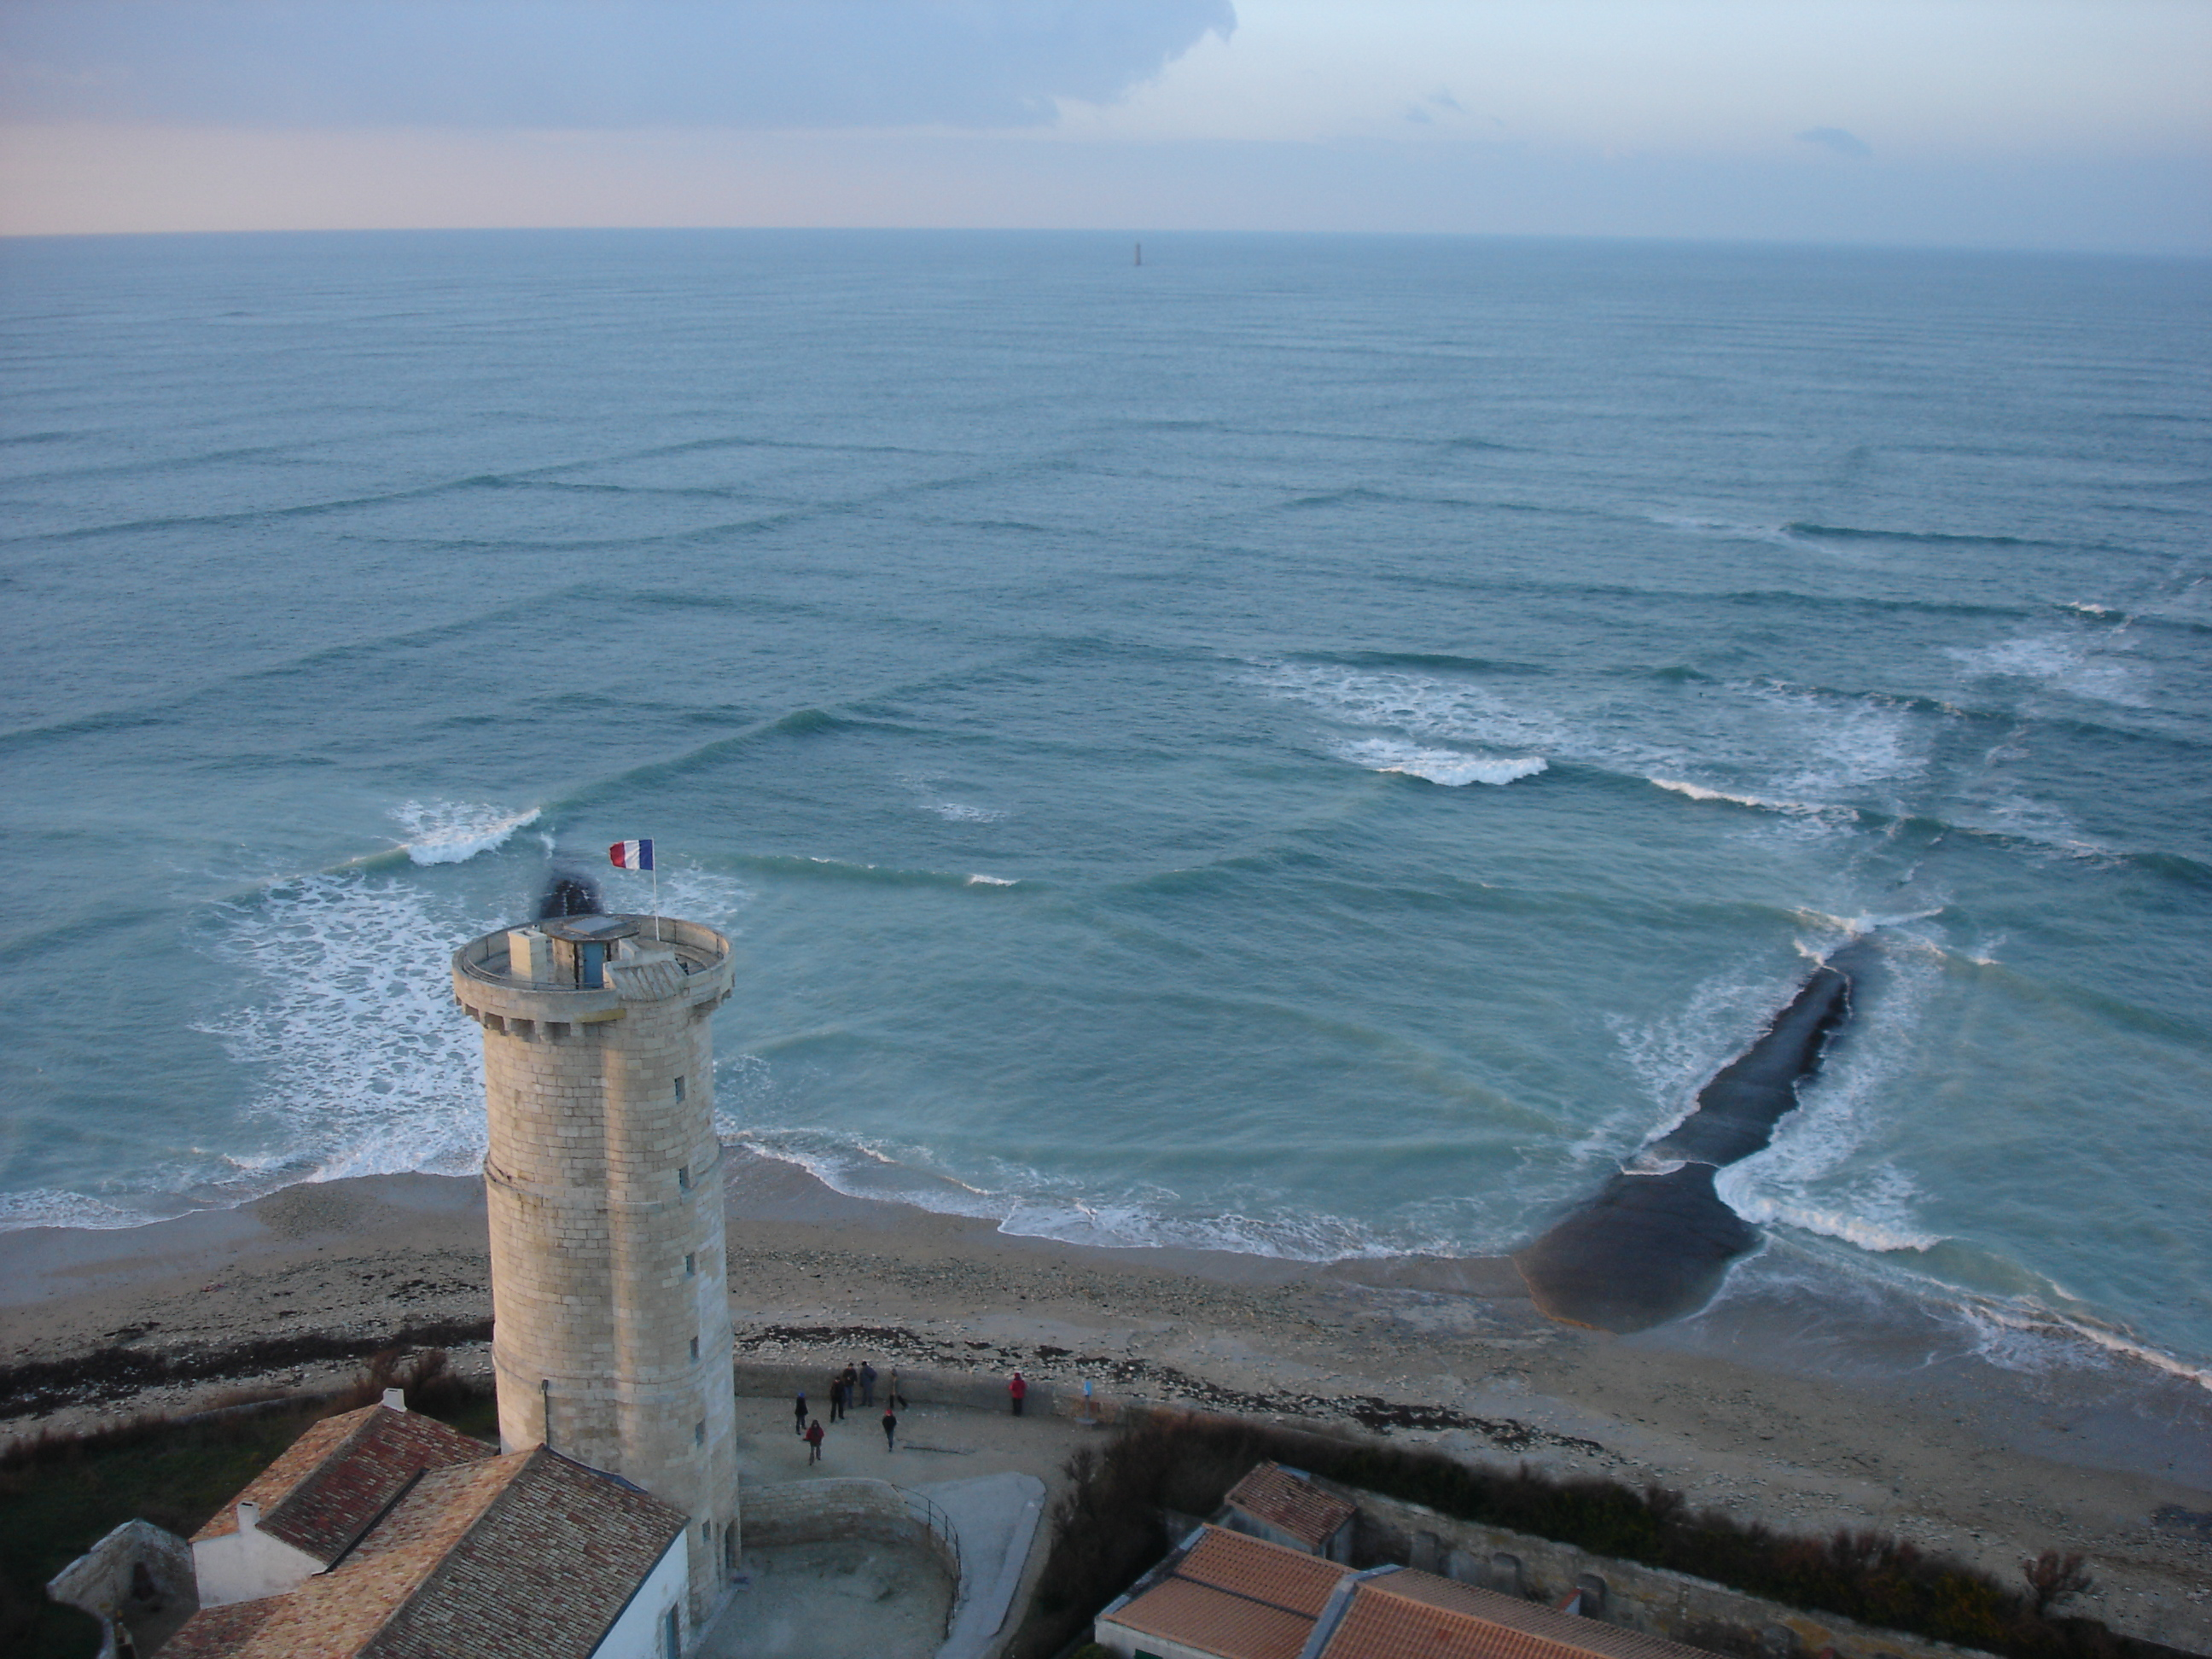
\includegraphics[width=\textwidth]{ile_de_re}
\vfill

\begin{center}
\texttt{Москва 1995}
\end{center}


\newpage




\section{Знакомство с главными героями}
\subsection{Якобианы кривых}

Пусть \( C \) --- компактная риманова поверхность рода \( g \). Это означает, в частности, что \( \dim_C H^0(C, \Omega_C^1) = g \), т. е. на кривой \( C \) имеется \( g \) линейно независимых над \( C \) голоморфных дифференциальных форм \( \omega_1, \ldots, \omega_g \). Кроме того, \( \operatorname{rk} H_1(C, \mathbb{Z}) = 2g \), и можно считать, что 
\( H_1(C, \mathbb{Z}) = \mathbb{Z}a_1 \oplus \cdots \oplus \mathbb{Z}a_g \oplus \mathbb{Z}b_1 \oplus \cdots \oplus \mathbb{Z}b_g \), 
а саму кривую \( C \) можно представить как результат склейки \( 4g \)-угольника в соответствии со схемой


\begin{figure}[h]
    \centering
    \input{images/scheme1.pdf_tex}
\end{figure}


Отметим на \( C \) некоторую точку \( P_0 \). Соединим, далее, произвольную точку \( P \) кривой \( C \) с \( P_0 \) каким-нибудь путем \( \gamma \) и проинтегрируем по этому пути формы \( \omega_1, \ldots, \omega_g \). Получим \( g \) комплексных чисел
\[
\int_{P_0}^{P} \omega_1, \ldots, \int_{P_0}^{P} \omega_g.
\]
Выбор пути \( \gamma \), разумеется, далеко не однозначен, но результат не изменится, если пути гомологичны. Если же пути отличаются на элемент \( \lambda \) из \( H_1(C, \mathbb{Z}) \), то к нашему \( g \)-мерному вектору добавится вектор значений интегралов от форм \( \omega_1, \ldots, \omega_g \) по \( \lambda \). Векторы
$
\left( \int_{\lambda} \omega_1, \ldots, \int_{\lambda} \omega_g \right)
$
с $\lambda \in H_1(C, \mathbb{Z})$
образуют в \( C^g \) решетку \( \Lambda \) ранга \( 2g \), называемую \emph{решеткой периодов}. Итак, мы получаем корректно определенное отображение \( j : C \to C^g / \Lambda \), называемое \emph{отображением Абеля}, при котором

\[
j(P) = \left( \int_{P_0}^{P} \omega_1, \ldots, \int_{P_0}^{P} \omega_g \right) + \Lambda.
\]

Легко сообразить, что это отображение не зависит от выбора начальной точки \( P_0 \). Факторгруппа \( \operatorname{Jac} C = C^g / \Lambda \) топологически является \( 2g \)-мерным тором и называется \textit{якобианом} кривой \( C \).

\textbf{Пример.} Если \( C \) есть эллиптическая кривая, т.е. её род равен 1, то \( \operatorname{Jac} C\) изоморфен \( C \) как комплексное многообразие. В частности, это позволяет определить на \( C \) групповую структуру.


Якобиан кривой, несмотря на простое топологическое устройство, несет важную информацию о ней: согласно теореме Торелли комплексные многообразия \( \operatorname{Jac} C \) и \( \operatorname{Jac} C' \) изоморфны тогда и только тогда, когда изоморфны кривые \( C \) и \( C' \).





\subsection{Проблема Шоттки}

Теперь естественно задать такой вопрос:

Имеется некоторый тор вида \( C^g / \Lambda \). Является ли он якобианом какой-нибудь кривой?

Риман нашел такие необходимые условия. Выберем базис \(\{a_i, b_i\}\) одномерных гомологий \(C\) так, чтобы выполнялись соотношения (в смысле формы пересечения):
\[
a_i \cdot b_j = \delta_{ij}, \quad a_i \cdot a_j = b_i \cdot b_j = 0 \text{ при } i \neq j,
\]
а базис \(\{\omega_i\}\) в \(H^0(C, \Omega_C^1)\) так, чтобы
\[
\int_{a_i} \omega_j = \delta_{ij}.
\]
Тогда интегралы по \(b\)-циклам составят \emph{матрицу периодов} \(B_{ij} = \int_{b_i} \omega_j\). Тор \(\operatorname{Jac} C\) есть фактор \(C^g / (\mathbb{Z}^g + B\mathbb{Z}^g)\). Риман доказал, что матрица \(B\) симметрична, а ее мнимая часть \(\operatorname{Im} B\) положительно определена. Кроме того, Риман обнаружил, что пространство модулей неособых комплексных кривых рода \(g\) при \(g > 1\) имеет размерность \(m_g = 3g - 3\), т. е. помимо дискретного параметра --- рода --- кривая может быть однозначно охарактеризована соответствующим числом непрерывных параметров --- «модулей». Как известно, при \(g = 1\) пространство модулей одномерно. Пространство же матриц \(B\), удовлетворяющих условиям Римана, имеет размерность \(r_g = \frac{g(g+1)}{2}\). Из сравнения размерностей вытекает, что далеко не всякий комплексный тор является чьим-то якобианом.

Решение проблемы было получено при малых \(g\):
\begin{itemize}
    \item при \(g = 1\) имеем \(m_1 = r_1 = 1\), и всегда \(\operatorname{Jac} C \cong C\);
    \item при \(g = 2\) имеем \(m_2 = r_2 = 3\), и все торы, удовлетворяющие условиям Римана, являются якобианами;
    \item при \( g = 3 \) имеем \( m_3 = r_3 = 6 \), и ситуация аналогична;
    \item при \( g = 4 \) имеем \( m_4 = 9 \), а \( r_4 = 10 \), и по гипотезе Фридриха Шоттки имеется одно соотношение на так называемые тэта-константы тора, выделяющее якобианы. Это соотношение было обнаружено Шоттки в 1888 г. ([Schot]). Его достаточность была доказана Игусой только в 1981 г. ([Igu]).

\end{itemize}


(Имеется в виду, что в случаях рода 2 и 3 соответствующие матрицы \( B \) являются неразложимыми, т. е. не приводятся целочисленными невырожденными преобразованиями к блочно-диагональному виду.)






\subsection{Солитонные уравнения}





















\end{document}
